% +--------------------------------------------------------------------+
% | Appendix A Page (Optional)                                         |
% +--------------------------------------------------------------------+

\cleardoublepage

\chapter{Guía de instalación para el servidor}
\label{app:guia_instalacion}

\section{Docker}
\label{app:docker}
Esta es una guía para el despliegue del servidor en Docker.

El repositorio del proyecto del servidor se encuentra en:
\url{https://github.com/ZReKoJ/Docker.git}

Para ello primero tenemos que tener docker instalado, el cual 
se puede instalar por el siguiente enlace \url{https://www.docker.com/}

Tras descargarse el repositorio, mediante commando, situarse en la carpeta raíz del proyecto.

\begin{lstlisting}[language=bash, caption=Despliegue de la instancia de docker]
    # Despliegue
    docker-compose up
\end{lstlisting}

Con la sentecia \textbf{docker-compose up} se despliega la instancia de docker con las configuraciones 
que están en el archivo docker-compose.yml.

Ahora que se ha levantado la instancia de docker y sus respectivos puertos mapeados.
Se conecta al container mediante ssh con la contraseña \textbf{tfg-ucm}

\begin{lstlisting}[language=bash, caption=Conexión ssh]
    # El puerto 22022 es el que se habia mapeado
    ssh root@localhost -p 22022
\end{lstlisting}

Una vez conectado al container, hay que ir a la ruta en el que se encuentra el proyecto: \url{/usr/src/app}

Antes de levantar el servicio, hay que preparar postgresql. El archivo SQL está dentro del proyecto
en el siguiente path: \url{/src/main/webapp/WEB-INF/sql/filmar_low.sql}. En la raíz del proyecto se 
encuentra un script llamado \textbf{database.sh}.

\begin{lstlisting}[language=bash, caption=Configuración postgresql]
    ./database.sh
\end{lstlisting}

Una vez configurado postgres, se procede al despliegue del servicio. Con \textbf{service.sh}.

\begin{lstlisting}[language=bash, caption=Despliegue]
    # Para parar el servicio
    ./service.sh start
    # Para reiniciar el servicio
    ./service.sh restart
    # Para parar el servicio
    ./service.sh
\end{lstlisting}

Ya está levantado el servicio en el puerto 8080, se puede probar con el siguiente enlace
\url{localhost:8080/films}.

\section{Heroku}
\label{app:heroku}
Para comenzar debemos crear una cuenta en \href{https://www.heroku.com/}{Heroku}.
Una vez la tenemos creamos una nueva aplicación a la
 cual daremos un nombre como vemos en la \autoref{fig:heroku_1} y este
 nombre a su vez será parte de la URL pública.
\begin{figure}[H]
    \centering
    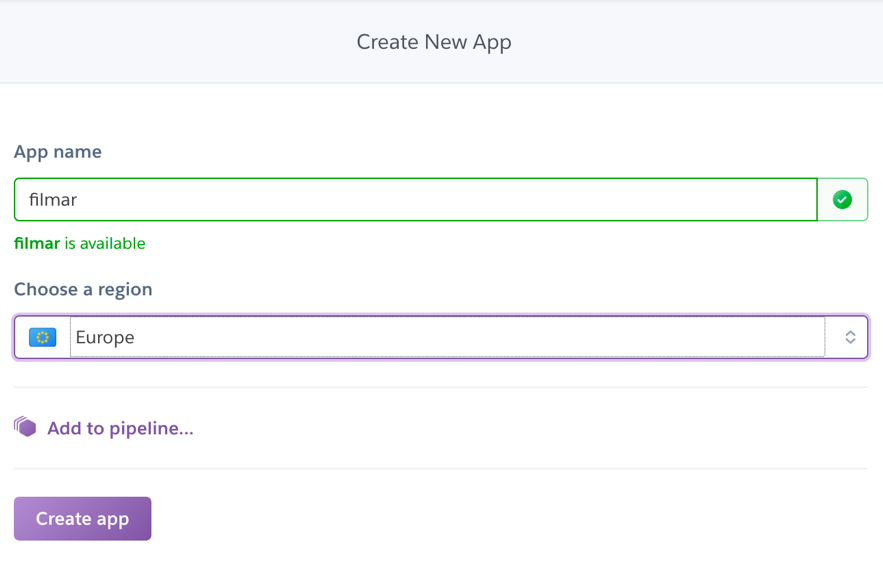
\includegraphics[width=6in]{figures/appendix-A/heroku_1.png}
    \caption{Crear nueva aplicación en Heroku}
    \label{fig:heroku_1}
\end{figure}
Cuando creemos la aplicación accederemos a la configuración en la que veremos
 opciones como en la figura \autoref{fig:heroku_2}.
\begin{figure}[H]
    \centering
    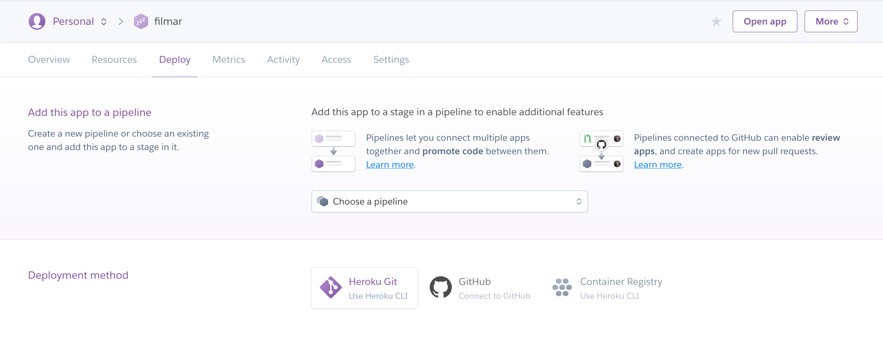
\includegraphics[width=6in]{figures/appendix-A/heroku_2.png}
    \caption{Configuración de la aplicación}
    \label{fig:heroku_2}
\end{figure}
Entramos en la pestaña de recursos y buscamos Postgres como vemos en la
\autoref{fig:heroku_3}. La seleccionamos y agregamos la versión gratuita.
\begin{figure}[H]
    \centering
    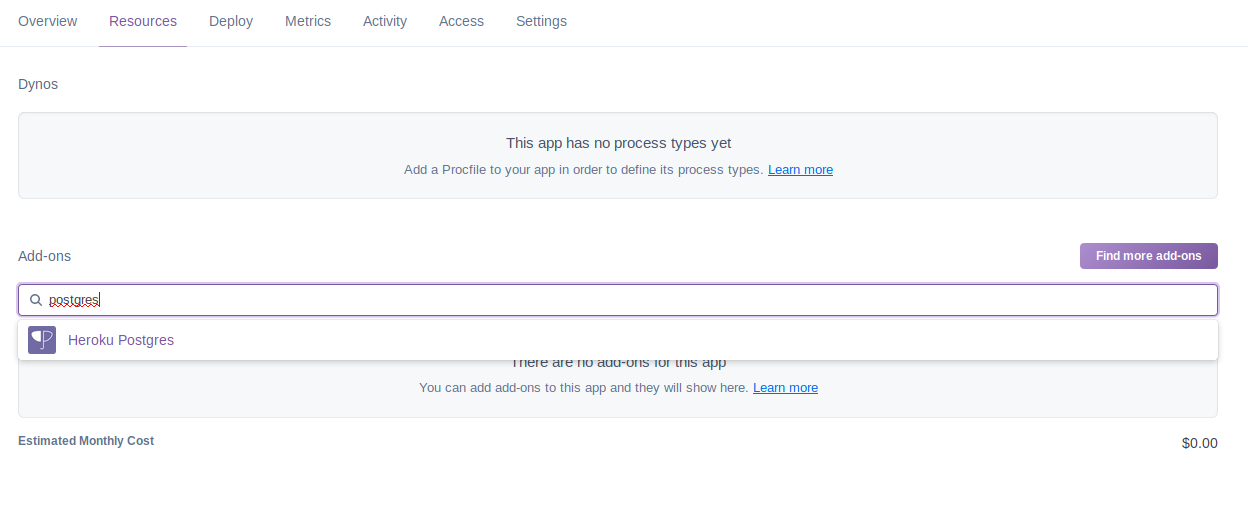
\includegraphics[width=6in]{figures/appendix-A/heroku_3.png}
    \caption{Añadir nuevos recursos}
    \label{fig:heroku_3}
\end{figure}
Si accedemos al recurso de la base de datos que acabamos de crear y Entramos
 en la configuración podemos ver las credenciales que necesitamos añadir a
 nuestro servidor para que funcione correctamente como vemos en la
 \autoref{fig:heroku_4}.
\begin{figure}[H]
    \centering
    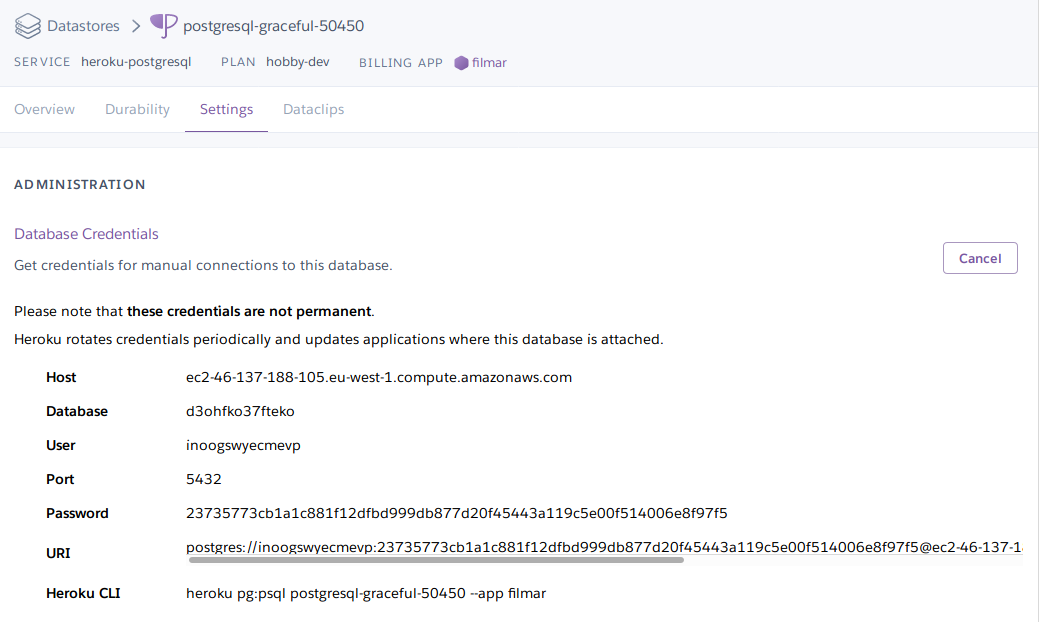
\includegraphics[width=6in]{figures/appendix-A/heroku_4.png}
    \caption{Ver credenciales}
    \label{fig:heroku_4}
\end{figure}
Si vamos a la pestaña de despliegue de la aplicación, como vemos en la
 \autoref{fig:heroku_5} nos ofrece diversos métodos de
 despliegue:
\begin{itemize}
    \item Heroku Git
    \item GitHub
    \item Container Registry
\end{itemize}
\begin{figure}[H]
    \centering
    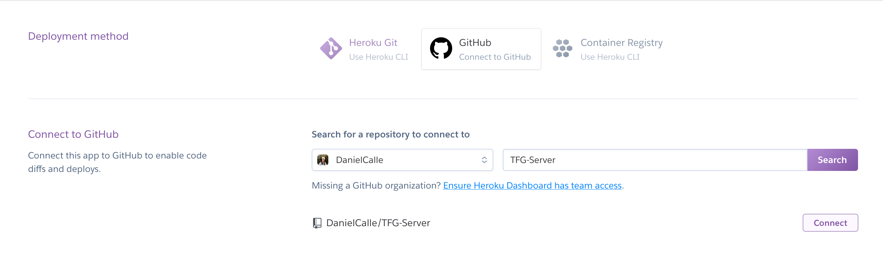
\includegraphics[width=6in]{figures/appendix-A/heroku_5.png}
    \caption{Métodos de despliegue}
    \label{fig:heroku_5}
\end{figure}
Elegimos la opción de GitHub que nos proporciona un despliegue fácil y rápido.
Tenemos que vincular la cuenta de nuestro GitHub (Importante ser el dueño del
 repositorio).
\begin{figure}[H]
    \centering
    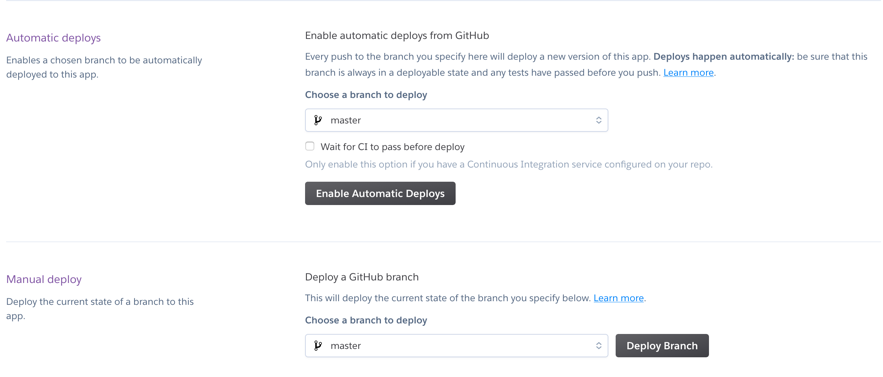
\includegraphics[width=6in]{figures/appendix-A/heroku_6.png}
    \caption{Opciones de despliegue utilizando Github}
    \label{fig:heroku_6}
\end{figure}
Una vez vinculada la cuenta de GitHub tenemos dos métodos de despliegue como
 vemos en la \autoref{fig:heroku_6}. Un método automático para desplegar los
 cambios de una rama del repositorio que se accionará cada vez que subamos
 cambios y otro método manual que se desplegará sólo cuando presionemos
 el botón. 
Cuando elijamos una de las opciones, la aplicación estará lista para usarse.